\documentclass[12pt]{amsart}
\usepackage{xeCJK} % 支持中文
\usepackage[margin=1in]{geometry}  % set the margins to 1in on all sides
\usepackage{amscd,latexsym,amsthm,amsfonts,amssymb,amsmath,amsxtra}
\usepackage{mathrsfs}
\usepackage[mathscr]{eucal}
\usepackage{hyperref}
\usepackage{pdfsync}
\usepackage[all,cmtip]{xy}
\usepackage{graphicx}
\usepackage{float}
\usepackage{color}
\usepackage{hyperref}[colorlinks,linkcolor=blue]
\usepackage{tikz}
\usepackage{tikz-cd}
\usetikzlibrary{decorations.pathreplacing}
\newcommand{\tikznode}[3][inner sep=0pt]{\tikz[remember
picture,baseline=(#2.base)]{\node(#2)[#1]{$#3$};}}
\usepackage{ytableau}


\setCJKmainfont{SimSun} % 设置中文字体,例如宋体
\setCJKsansfont{Microsoft YaHei} % 设置无衬线字体,例如微软雅黑
\setCJKmonofont{FangSong} % 设置等宽字体,例如仿宋
\numberwithin{equation}{section}
\pagestyle{plain}
\setcounter{secnumdepth}{5}

\pagestyle{headings}
\renewcommand\theequation{\thesection.\arabic{equation}}

%%%%%%%%%%%%%%%%%%%%%%%%%%%%%%%%%%%%%%%%%%%%%% Theorem style

\newtheorem{thm}{Theorem}[section]
\newtheorem{cor}[thm]{Corollary}
\newtheorem{prop}[thm]{Proposition}
\newtheorem{lem}[thm]{Lemma}
\newtheorem{assump}[thm]{Assumption}
\newtheorem{conj}[thm]{Conjecture}
\newtheorem{rk}[thm]{Remark}
\newtheorem{question}[thm]{Question}
\newtheorem{defn}[thm]{Definition}
\newtheorem{con}[thm]{Construction}
\newtheorem{examp}[thm]{Example}
\newtheorem{notn}[thm]{Notation}
\newtheorem{exer}[thm]{Exercise}

%%%%%%%%%%%%%%%%%%%%%%%%%%%%% Bold Fonts

\newcommand{\BA}{{\mathbb {A}}}
\newcommand{\BB}{{\mathbb {B}}}
\newcommand{\BC}{{\mathbb {C}}}
\newcommand{\BD}{{\mathbb {D}}}
\newcommand{\BE}{{\mathbb {E}}}
\newcommand{\BF}{{\mathbb {F}}}
\newcommand{\BG}{{\mathbb {G}}}
\newcommand{\BH}{{\mathbb {H}}}
\newcommand{\BI}{{\mathbb {I}}}
\newcommand{\BJ}{{\mathbb {J}}}
\newcommand{\BK}{{\mathbb {U}}}
\newcommand{\BL}{{\mathbb {L}}}
\newcommand{\BM}{{\mathbb {M}}}
\newcommand{\BN}{{\mathbb {N}}}
\newcommand{\BO}{{\mathbb {O}}}
\newcommand{\BP}{{\mathbb {P}}}
\newcommand{\BQ}{{\mathbb {Q}}}
\newcommand{\BR}{{\mathbb {R}}}
\newcommand{\BS}{{\mathbb {S}}}
\newcommand{\BT}{{\mathbb {T}}}
\newcommand{\BU}{{\mathbb {U}}}
\newcommand{\BV}{{\mathbb {V}}}
\newcommand{\BW}{{\mathbb {W}}}
\newcommand{\BX}{{\mathbb {X}}}
\newcommand{\BY}{{\mathbb {Y}}}
\newcommand{\BZ}{{\mathbb {Z}}}
\newcommand{\bi}{{\mathbf {i}}}
%%%%%%%%%%%%%%%%%%%%%%%%%%%%%%%%%%%%%%%% Curly Fonts

\newcommand{\CA}{{\mathcal {A}}}
\newcommand{\CB}{{\mathcal {B}}}
\newcommand{\CC}{{\mathcal {C}}}
%\newcommand{\CD}{{\mathcal {D}}}
\newcommand{\CE}{{\mathcal {E}}}
\newcommand{\CF}{{\mathcal {F}}}
\newcommand{\CG}{{\mathcal {G}}}
\newcommand{\CH}{{\mathcal {H}}}
\newcommand{\CI}{{\mathcal {I}}}
\newcommand{\CJ}{{\mathcal {J}}}
\newcommand{\CK}{{\mathcal {K}}}
\newcommand{\CL}{{\mathcal {L}}}
\newcommand{\CM}{{\mathcal {M}}}
\newcommand{\CN}{{\mathcal {N}}}
\newcommand{\CO}{{\mathcal {O}}}
\newcommand{\CP}{{\mathcal {P}}}
\newcommand{\CQ}{{\mathcal {Q}}}
\newcommand{\CR}{{\mathcal {R}}}
\newcommand{\CS}{{\mathcal {S}}}
\newcommand{\CT}{{\mathcal {T}}}
\newcommand{\CU}{{\mathcal {U}}}
\newcommand{\CV}{{\mathcal {V}}}
\newcommand{\CW}{{\mathcal {W}}}
\newcommand{\CX}{{\mathcal {X}}}
\newcommand{\CY}{{\mathcal {Y}}}
\newcommand{\CZ}{{\mathcal {Z}}}

%%%%%%%%%%%%%%%%%%%%%%%%%%%%%%%%%%%%%%%% Roman Fonts

\newcommand{\RA}{{\mathrm {A}}}
\newcommand{\RB}{{\mathrm {B}}}
\newcommand{\RC}{{\mathrm {C}}}
\newcommand{\RD}{{\mathrm {D}}}
\newcommand{\RE}{{\mathrm {E}}}
\newcommand{\RF}{{\mathrm {F}}}
\newcommand{\RG}{{\mathrm {G}}}
\newcommand{\RH}{{\mathrm {H}}}
\newcommand{\RI}{{\mathrm {I}}}
\newcommand{\RJ}{{\mathrm {J}}}
\newcommand{\RK}{{\mathrm {K}}}
\newcommand{\RL}{{\mathrm {L}}}
\newcommand{\RM}{{\mathrm {M}}}
\newcommand{\RN}{{\mathrm {N}}}
\newcommand{\RO}{{\mathrm {O}}}
\newcommand{\RP}{{\mathrm {P}}}
\newcommand{\RQ}{{\mathrm {Q}}}
\newcommand{\RR}{{\mathrm {R}}}
\newcommand{\RS}{{\mathrm {S}}}
\newcommand{\RT}{{\mathrm {T}}}
\newcommand{\RU}{{\mathrm {U}}}
\newcommand{\RV}{{\mathrm {V}}}
\newcommand{\RW}{{\mathrm {W}}}
\newcommand{\RX}{{\mathrm {X}}}
\newcommand{\RY}{{\mathrm {Y}}}
\newcommand{\RZ}{{\mathrm {Z}}}
\renewcommand{\Re}{{\mathrm {Re}}}
\newcommand{\Ri}{{\mathrm {i}}}
\newcommand{\Ann}{{\mathrm{Ann}}}
%%%%%%%%%%%%%%%%%%%%%%%%%%%%%%%%%%%%%%%%%%  Gothic Fonts, Lie algebras

\newcommand{\fa}{\mathfrak{a}}
\newcommand{\fb}{\mathfrak{b}}
\newcommand{\fc}{\mathfrak{c}}
\newcommand{\fg}{\mathfrak{g}}
\newcommand{\fh}{\mathfrak{h}}
\newcommand{\fk}{\mathfrak{k}}
\newcommand{\fl}{\mathfrak{l}}
\newcommand{\fm}{\mathfrak{m}}
\newcommand{\fn}{\mathfrak{n}}
\newcommand{\fo}{\mathfrak{o}}
\newcommand{\fp}{\mathfrak{p}}
\newcommand{\fq}{\mathfrak{q}}
\newcommand{\fr}{\mathfrak{r}}
\newcommand{\fs}{\mathfrak{s}}
\newcommand{\ft}{\mathfrak{t}}
\newcommand{\fu}{\mathfrak{u}}
\newcommand{\fv}{\mathfrak{v}}
\newcommand{\fy}{\mathfrak{y}}
\newcommand{\fz}{\mathfrak{z}}
\newcommand{\fgl}{{\mathfrak{gl}}}
\newcommand{\fsl}{{\mathfrak{sl}}}
\newcommand{\fso}{{\mathfrak{so}}}
\newcommand{\fsp}{{\mathfrak{sp}}}
\newcommand{\fsu}{{\mathfrak{su}}}

%%%%%%%%%%%%%%%%%%%%%%%%%%%%%%%%%% Algebraic Groups and Representation

\newcommand{\GL}{{\mathrm{GL}}}
\newcommand{\SL}{{\mathrm{SL}}}
\newcommand{\SU}{{\mathrm{SU}}}
\newcommand{\GU}{{\mathrm{GU}}}
\newcommand{\SO}{{\mathrm{SO}}}
\newcommand{\GO}{{\mathrm{GO}}}
\newcommand{\Sp}{{\mathrm{Sp}}}
\newcommand{\GSp}{{\mathrm{GSp}}}
\newcommand{\quo}{\backslash}
\newcommand{\adequo}[1]{#1(\F)\quo #1(\mathds{A})}
\newcommand{\ade}[1]{#1(\mathds{A})}
\newcommand{\Hom}{{\mathrm{Hom}}}
\newcommand{\Bil}{{\mathrm{Bil}}}
\newcommand{\Id}{{\mathrm{Id}}}\newcommand{\id}{{\mathrm{id}}}
\newcommand{\Ind}{{\mathrm{Ind}}}
\newcommand{\Irr}{{\mathrm{Irr}}}
\newcommand{\End}{{\mathrm{End}}}
\newcommand{\Aut}{{\mathrm{Aut}}}
\newcommand{\Inn}{{\mathrm{Inn}}}
\newcommand{\Out}{{\mathrm{Out}}}
\newcommand{\Ad}{{\mathrm{Ad}}}
\newcommand{\ad}{{\mathrm{ad}}}
\newcommand{\Der}{{\mathrm{Der}}}
\newcommand{\Lie}{{\mathrm{Lie}}}
\newcommand{\Mat}{{\mathrm{Mat}}}
\newcommand{\sgn}{{\mathrm{sgn}}}
\newcommand{\Rep}{{\mathrm{Rep}}}
\newcommand{\ten}{\otimes}
\newcommand{\proten}{\hat{\otimes}}
\newcommand{\Mell}[1]{\mathcal{M}#1}
\newcommand{\Gal}[1]{\Gamma_{#1}}
\newcommand{\Tr}{{\mathrm{Tr}}}
\newcommand{\gr}{{\mathrm{gr}}}
\newcommand{\Sym}{{\mathrm{Sym}}}
\newcommand{\diag}{\mathrm{diag}}


%%%%%%%%%%%%%%%%%%%%%%%%%%%%%%%%%   Math formula

\newcommand{\sbst}{\subseteq}
\newcommand{\norm}[1]{\lVert#1\rVert}
\newcommand{\abs}[1]{\lvert#1\rvert}
\newcommand{\set}[2]{\{#1\,|\,#2\}}
\newcommand{\bigset}[2]{\Biggl\{#1\,\bigg\lvert\,#2\Biggr\}}
\newcommand{\defmap}[5]{
           \begin{equation*}
              \begin{aligned}
                   #1:\quad  & #2 &\longrightarrow &\quad #3 \\
                      \quad  & #4    &\longmapsto  &\quad #5
              \end{aligned}
           \end{equation*}
          }
\newcommand{\mtrtwo}[4]{\begin{pmatrix} #1 &#2 \\#3 &#4 \end{pmatrix}}
\newcommand{\mtrthr}[9]{\begin{pmatrix} #1 &#2 &#3 \\#4 &#5 &#6\\ #7 &#8 &#9 \end{pmatrix}}
\newcommand{\defmtrtwo}[6]{
           \begin{equation*}
               #1 = \bigset{\mtrtwo{#2}{#3}{#4}{#5}}{#6},
           \end{equation*}
           }
\newcommand{\shortexact}[5]{#1\rightarrow #2 \rightarrow #3 \rightarrow #4\rightarrow #5}
\renewcommand{\bar}{\overline}
\renewcommand{\tilde}{\widetilde}
\newcommand{\eps}{\epsilon}

\author{Idle}
\begin{document}
\ytableausetup{centertableaux}
\title[Notes]{Notes}
\maketitle
\begin{figure}
  \centering
  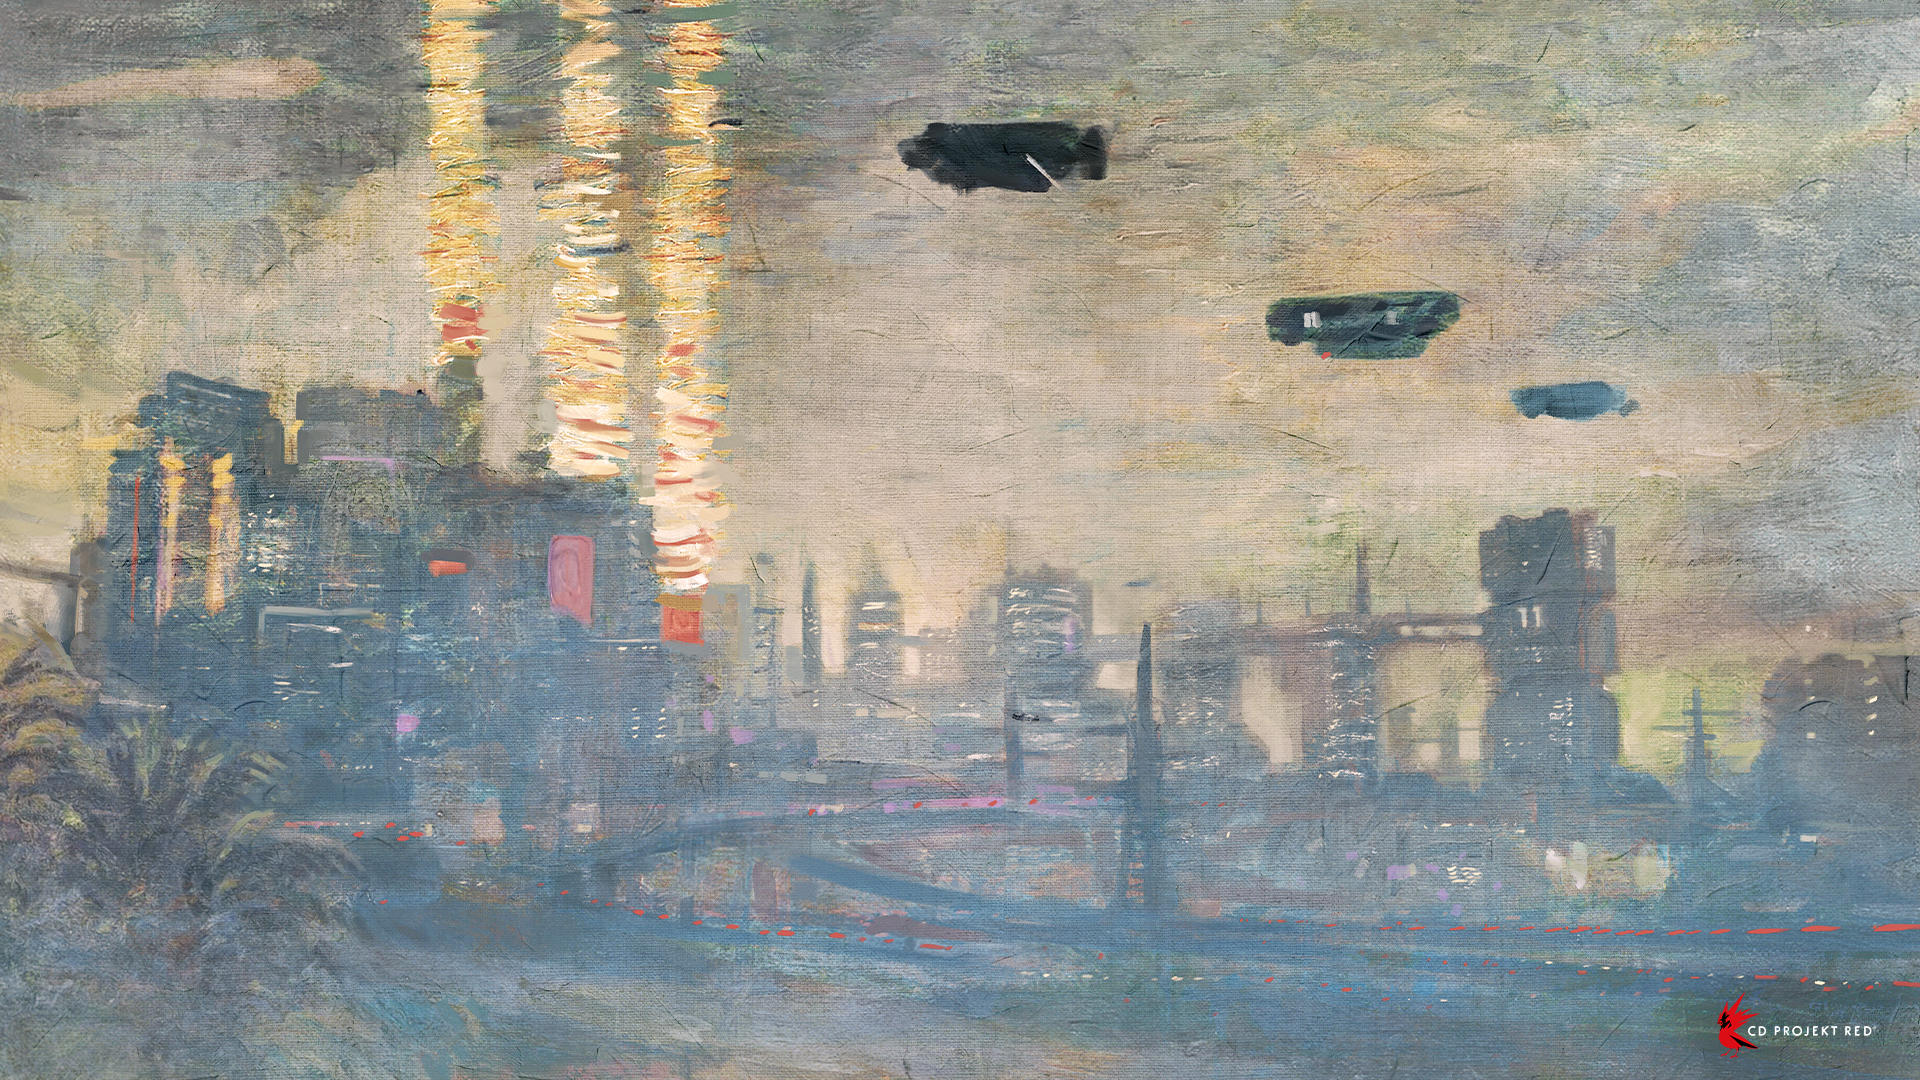
\includegraphics[width=1.0\linewidth]{Claude_Monet-NC.jpg}
  \caption{Night City}
  \label{night City}
\end{figure}

Hello!


This note is mainly used to record some trivial
but interesting problems that I encounter
in daily life.



For as the heavens are higher than the earth, so are my ways higher than your ways and my thoughts than your thoughts.---Isaiah 55:9

\newpage


\tableofcontents

\newpage

\section{2023.12.22}\label{1}

\subsection{Identification of co-character groups with Lie algebras}
Settings: $G$ complex connected reductive algebraic group, fix a splitting datum
$(B,H,\{X_\alpha\})$.


There is an identification \defmap{I}{X_*(H)\otimes \BC}{\fh}{\phi}{d\phi(1)}


The weight lattice for $G$ is $P = \set{\lambda \in X^*(H)\otimes \BC}{\langle \lambda, \check{\alpha} \rangle \in \BZ \ \textrm{for all} \ \alpha \in \Delta }$


The co-weight lattice is $\check{P} = \set{\check{\lambda} \in X_*(H)\otimes \BC}{\langle\alpha , \check{\lambda} \rangle \in \BZ \ \textrm{for all } \ \check{\alpha} \in \check{\Delta}}$



Under this identification we have

\begin{align*}
  \set{\check{\lambda} & \in \fh}{exp(\check{\lambda})=0}                                                                                                        \\
                       & = \set{\check{\lambda} \in X_*(H)\otimes \BC}{\phi(exp(d \check{\lambda}(1))) = 1 \ \textrm{for all} \ \phi \in X^*(H)}                 \\
                       & = \set{\check{\lambda} \in X_*(H)\otimes \BC}{exp(\langle\phi,\check{\lambda} \rangle) = 1 \ \textrm{for all } \ \phi \in X^*(H)}       \\
                       & = \set{\check{\lambda} \in X_*(H)\otimes \BC}{\langle\phi,\check{\lambda} \rangle \in 2 \pi i \BZ \ \textrm{for all} \ \phi \in X^*(H)} \\
                       & = 2 \pi i X_*(H).
\end{align*}
And similarly
$$\check{P} = \set{\check{\lambda} \in \fh}{exp(2 \pi i \check{\lambda}) \in Z(G)} $$


There is also an identification
\defmap{J}{X^*(H)\otimes \BC}{\fh ^*}{\varphi}{d \varphi}

Under this identification ...  I forget what I want to say.

\subsection{Pinnings of algebraic groups}

\begin{thm}[see AdC18]
  Inner automorphism group $\mathrm{Inn(G)}$ of $G$ is equal to $\mathrm{G/Z(G)}$,
  $\mathrm{Inn(G)}$ acts freely and transitively on the set of pinnings.
\end{thm}


I know that there is an analogy in compact connected groups, and it has been proved.

\begin{thm}
  If $\RG$ is a compact connected group, then its inner automorphism group $\mathrm{Inn(G)} = \mathrm{G/Z(G)}$
  acts freely and transitively on the set of pinnings.
  (where pinnings for it is a bit different from the complex case, that $(T, B_\BC,\mathcal{X})$
  is a pinning if $T$ is a maximal torus, $B_\BC$ a Borel of $G_\BC$ containing $T$, $\mathcal{X}$
  is a set of real rays in simple root space.)
\end{thm}

\begin{proof}
  Here's proof from mathoverflow \href{https://mathoverflow.net/questions/377981/classification-of-not-necessarily-connected-compact-lie-groups/378141#378141}{Lspise's answer}:
  \begin{figure}[H]
    \centering
    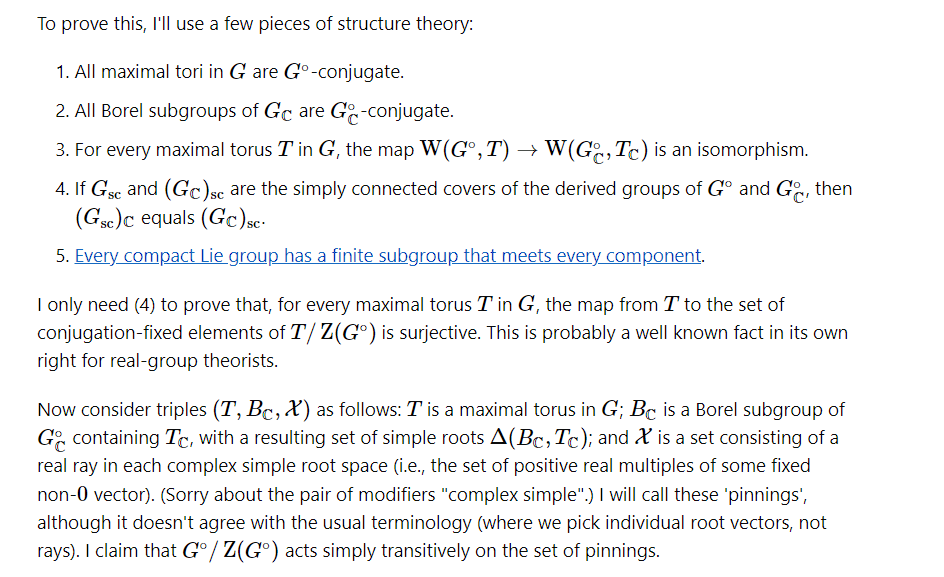
\includegraphics[width=1.0\linewidth]{1.png}
  \end{figure}

  \begin{figure}[H]
    \centering
    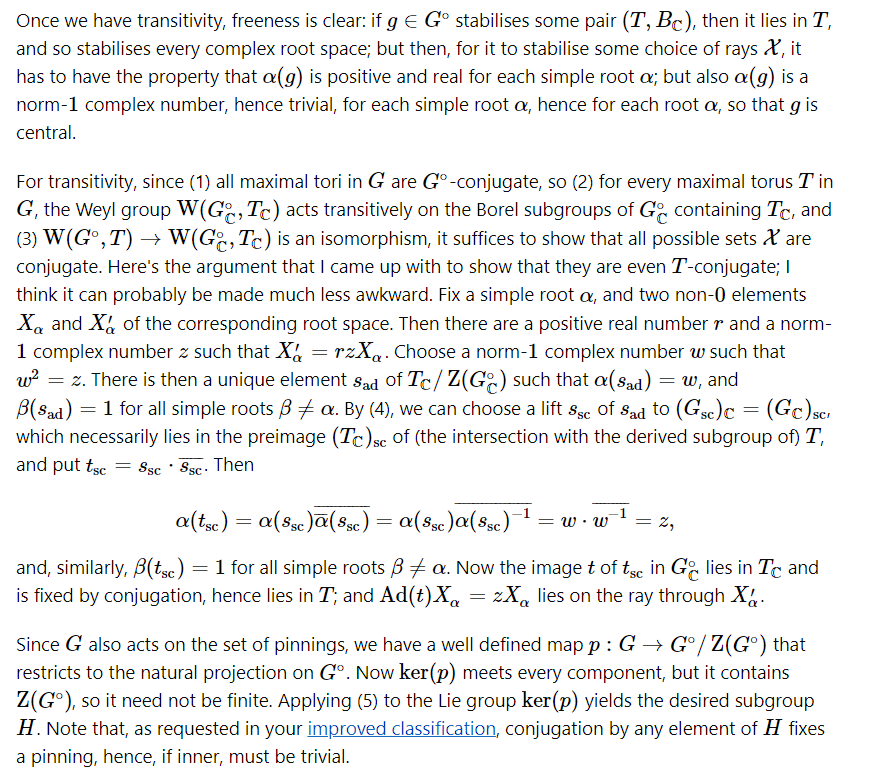
\includegraphics[width=1.0\linewidth]{2.png}
  \end{figure}
\end{proof}

\newpage

\begin{rk}
  The pinnings show that split reductive algebraic groups look like butterflies!
\end{rk}

\begin{figure}[H]
  \centering
  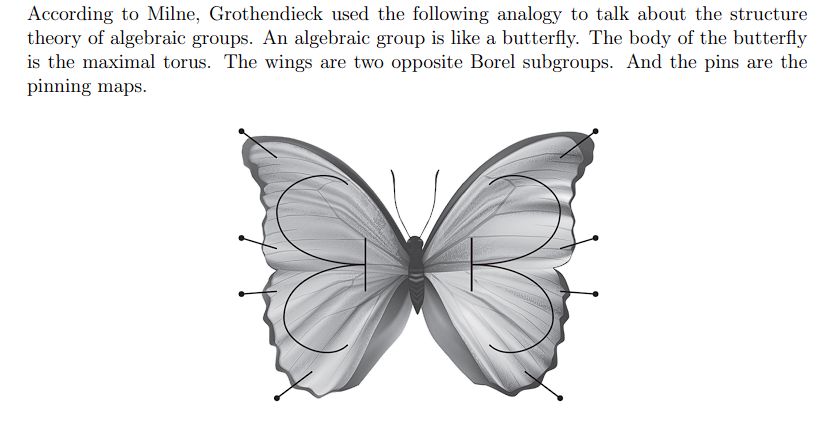
\includegraphics[width=1.0\linewidth]{3.png}
  \caption{Pinning of butterfly}
\end{figure}

\newpage

\subsection{Coherent continuation representations}

Until the end of today, $G$ denotes a real reductive group in Harish-Chandra class.

Let's recall some basic definitions of coherent continuation representations, in order
for me to do calculations in the case of real classical groups.


Fix a connected reductive complex Lie group $G_\BC$, together with a Lie group homomorphism
$\mathrm{\iota: G \to  G_\BC}$ such that its differential $\mathrm{d\iota} : \mathrm{Lie(G)} \to \mathrm{Lie(G_\BC)}$
has the following two properties:
\begin{enumerate}
  \item the kernel of $\mathrm{d\iota}$ is contained in the center of $\mathrm{Lie(G)}$;
  \item the image of $\mathrm{d\iota}$ is a real form of $\mathrm{Lie(G)}$.
\end{enumerate}

The analytical weight lattice of $\mathrm{G_\BC}$ is identified with a subgroup of $^{a}\fh^*$ via $\mathrm{d\iota}$.
We write $Q_\iota \subset \  ^{a}\fh^*$ for this subgroup. Denote root lattice by $Q_\fg$,
weight lattice by $Q^\fg$, then $$Q_\fg \subset Q_\iota \subset Q^\fg.$$
They are all $W$ stable subgroups.
And we have some categories:
\begin{enumerate}
  \item $\mathrm{Rep}(\fg,Q_\iota)$ the category of all finite-dimensional representations of $\fg$ whose weight are contained in $Q_\fg$, \textcolor{red}{it can be identified with $\mathrm{Rep(Lie(G_\BC),Q_\iota)}$ and hence $\mathrm{Rep_{finite}(G_\BC)}$};
  \item $\mathrm{Rep(G)}$ the category of all Casselman-Wallach representations of $G$, and its full subcategories $\mathrm{Rep_\mu(G)}$, $\mathrm{Rep_S(G)}$.
\end{enumerate}
To denote their Grothendieck groups, we replace $\mathrm{Rep}$ by $\mathcal{K}$.


Fix a $Q_\iota$-coset $\Lambda = \lambda + Q_\iota \subset \  ^{a}\fh^*$.


\begin{defn}[coherent family]
  A $\mathcal{K}(G)$-valued $\Lambda$ coherent family is a map
  $$\varPhi : \Lambda \to \mathcal{K}(G)$$
  satisfies the following two conditions:
  \begin{enumerate}
    \item for all $\nu \in \Lambda$, $\varPhi(\nu) \in \mathcal{K}_{\nu}(G)$;
    \item for all representations $F \mathrm{ \in Rep}(\fg,Q_\iota)$ and all $\nu \in \Lambda$,
          $$F \cdot (\varPhi(\nu)) = \sum\limits_{\mu} \varPhi(\nu + \mu),$$
          where $\mu$ runs over all weights of $\mathrm{F}$, counted with multiplicities.
  \end{enumerate}
  The set of coherent families is denoted by $\mathrm{Coh}_\Lambda(\mathcal{K}(G))$
\end{defn}
We have the integral Weyl group $W_{\Lambda} = \set{w \in W}{w\lambda - \lambda \in Q_\iota}$
there is a representation of $W_\Lambda$ on $\mathrm{Coh}_\Lambda(\mathcal{K}(G))$ by
$$(w \cdot \varPhi)(\nu) = \varPhi (w^{-1}\nu).$$
This is called a coherent continuation representation.

\newpage


\section{2023.12.23}\label{2}

\subsection{Review of regular parameter}

Following yesterday's discussion of coherent continuation representations, we define two basis
for it, use Langland classification.

Suppose $H$ is a Cartan subgroup of $G$, by which we mean a subgroup that is the centralizer of
a Cartan subalgebra of $\Lie(G)$ \textcolor{yellow}{(In the case of linear groups, it's just a
  real algebraic torus.)}. $H$ has a unique maximal compact subgroup (since $G$ is in Harish-Chandra's
class, adjoint representation of $H$ is trivial, $H_0$ lies in the center of $H$, as we know, all
maximal subgroups of Lie groups are conjugate to each other, use Cartan decomposition of $H$, we win. In fact,
$H$ has a unique maximal compact torus and a unique maximal split torus)
We denote by $\Delta_{\fh} \subset \fh^*$ the root system of $\fg$. A root is called imaginary
if $\check{\alpha } \in \ft$ (i.e. roots which take pure imaginary values on $\Lie(H)$), an imaginary root $\alpha$ is
called compact if $\fg_{\alpha}$ and $\fg_{-\alpha}$ is contained in the complexified Lie algebra of a common compact subgroup of $G$.(this is equivalent to $\fg_\alpha $ belong to a Lie subalgebra of a compact subgroup, since $\fg_\alpha $ lies in a Lie subalgebra of maximal compact subgroup is equivalent to $\fg_{-\alpha }$ Lies in the same subgroup)


There are two important facts about the representation theory of $H$:
\begin{enumerate}
  \item Every Casselman-Wallach representation of $H$ is finite-dimensional, it follows directly from that $H$ is an extension of an abelian group and a finite group;
  \item For every $\Gamma \in \mathrm{Irr(H)}$ differential of $\Gamma$ is a direct sum of one-dimensional representations attached to a unique $\mathrm{d\Gamma \in \fh^*}$.
        (it is true because $H$ is in Harish-Chandra's class).
\end{enumerate}


For every Borel subalgebra $\fb$ of $\fg$ containing $\fh$, write 
$$\xi_{\fb}: \fh \to \ ^{a}\fh,$$
for the linear isomorphism attached to $\fb$ defined by 
$$\fh \hookrightarrow  \fb \to \fb / [\fb,\fb] = \ {^{a}\fh}.$$
The transpose inverse of this map is still denoted by $\xi_{\fb}: \ ^{a}\fh^* \to \fh^*$.\\


Write $$W(^{a}\fh^*,\fh^*) :=  \set{\xi_{\fb}: \ ^{a}\fh^* \to \fh^*}{\fb \ \textrm{is a Borel subalgebra containing} \ \fh}.$$

\begin{defn}
  For every element $\xi \in W(^{a}\fh^*,\fh^*)$, put
  $$\delta(\xi) := \frac{1}{2} \cdot \sum\limits_{\alpha  \ \textrm{is an imaginary root in} \ \xi\Delta^+}\alpha - \sum\limits_{\beta \ \textrm{is an compact imaginary root in} \ \xi\Delta^+}\beta \in \fh^* .$$
  Write $\mathcal{P} _{\Lambda}(G)$ for the set of all triples $\gamma = (H,\xi,\Gamma)$, where
  $H$ is a Cartan subgroup of $G$, $\xi \in W(^{a}\fh^*,\fh^*)$, and
  \defmap{\Gamma}{\Lambda}{\mathrm{Irr(H)}}{\nu}{\Gamma_{\nu}}
  is a map with the following properties:
  \begin{enumerate}
    \item $\Gamma_{\nu+\beta} = \Gamma_{\nu} \otimes \xi(\beta)$ for all $\beta \in Q_{\iota}$ and $\nu \in \Lambda$;
    \item $\mathrm{d\Gamma_{\nu}} = \xi(\nu) + \delta(\xi)$ for all $\nu \in \Lambda$.\textcolor{red}{(note that Cartan subgroups not always have irr repn with this differential!)}
  \end{enumerate}
  Here $\xi(\beta)$ is naturally viewed as a character of $H$ by using the homomorphism
  $\iota : H \to H_{\BC}$, and $H_{\BC}$ is a Cartan subgroup of $G_{\BC}$ containing $\iota(H)$.
\end{defn}

\newpage

\subsection{Outer automorphism of algebraic groups}

\begin{lem}[a simple discover of abstract algebra]
  $G$ an abstract group, $H$ a normal subgroup of $G$, if $G$ acts
  transitively on a set $X$ such that the restriction of this action
  to $H$ is free and transitive, then the short exact sequence of groups
  $$\shortexact{1}{H}{G}{G/H}{1}$$
\end{lem}

\begin{proof}
  Actually choose an element $x \in X$, we have
  $$ G \simeq \mathrm{Stab}_{G}(x) \ltimes H.$$
\end{proof}


Using this lemma, we can see that for a complex connected reductive
algebraic group $G$, $\Aut(G)$ acts on the set of pinnings transitively,
with its normal subgroup the $\Inn(G)$ acts freely and transitively,
so every pinning gives us a split of the short exact sequence
$$\shortexact{1}{\Inn(G)}{\Aut(G)}{\Out(G)}{1}.$$


Some facts about split connected reductive algebraic groups over arbitrary field $k$:
\begin{enumerate}
  \item $\{ \textrm{split connected reductive algebraic groups} \}/_\backsim \ = \{ \textrm{root datums}\} /_\backsim $;
  \item For any two automorphisms of $G$, if they induce the same automorphism of root datum, then they differ by an inner automorphism;
  \item Fix a pinning, we get an isomorphism $\Out(G) \simeq \Aut(D_b)$.
\end{enumerate}


\newpage


\section{2023.12.26}\label{3}

\begin{thm}[Harish-Chandra's parameter of discrete series repn]
  $G$ be a connected semisimple Lie group (maybe there is an analogy for real reductive group), $K$ a maximal torus of $G$, suppose that
  $\mathrm{rank}(K) = \mathrm{rank}(G)$, fix a compact maximal torus $T \in K$ and positive system $\Delta^+$. Then for any analytically integral weight $\lambda + \rho$, there exist a discrete series representation $\pi_{\lambda}$, such that:
  \begin{enumerate}
    \item The infinitesimal character of $\pi_\lambda$ is $\lambda$;
    \item $\nu = \lambda + \rho - 2\rho_c$ is the highest weight of a minimal  $K$ type of $\pi_\lambda$;
    \item If $\mu$ is any highest weight of irreducible $K$ representation exist in $\pi_\lambda$, then $$\mu = \nu + \sum\limits_{\alpha \in \Delta^+} n_{\alpha}\alpha$$.
  \end{enumerate}
  Moreover, $\pi_{\lambda} \simeq \pi_{\lambda'}$ if and only if $\lambda$ and $\lambda'$ lies in the same $W_c$ orbit.
\end{thm}

In the above theorem, $\rho - 2\rho_c$ is canonically realized as a continuous character of double cover of $T$, called $\tilde{T} $, which can be realized as a pull-back diagram:
\begin{tikzcd}
  \tilde{T} \arrow[r] \arrow[d] & \BC^\times \arrow[d,"z \mapsto z^2"] \\
  T \arrow[r,"2\rho - 4\rho_c"] & \BC^\times
\end{tikzcd}


Similarly, $\lambda$ is also a character of a double cover of $T$, with respect to $-2\lambda$, but the difference of $-2\lambda$ and $2\rho - 4\rho_c$ is a square of a character of $T$, the two double covers are canonically isomorphic.

\textcolor{red}{In fact, there is a one to one correspondence! Which I finally get it}:

$$\{ \textrm{genuie characters of} \ \tilde{T}_{\rho_{im}}    \} \simeq \set{(\Gamma,\nu) \in X^*(T) \times \ft^*}{d\Gamma = \nu + \rho_{im}-2\rho_{im,c}}. $$
The correspondence is given by

\begin{align*}
  \chi         & \mapsto (\chi  \otimes (\rho_{im}-2\rho_{im,c}),d\chi) \\
  (\Gamma,\nu) & \mapsto \Gamma \otimes (2\rho_{im,c} - \rho_{im})
\end{align*}

\begin{defn}[Langlands parameter]
  Let $G$ be a linear real reductive group, the Langlands parameters for $G$ is a triple $(H,\gamma,R_{i\BR}^+)$. Such that
  \begin{enumerate}
    \item $\mathrm{Hladk\acute{y}}$ \'{a}
  \end{enumerate}
\end{defn}

\newpage

\section{2024.2.27}\label{4}
Today, I learned how to draw the Young tableau.

\begin{ytableau}
  \none[2] &  &  & \none \\
  \none[1]  &  &  &  \\
  \none & \none[1] & \none[2] & \none[3]
\end{ytableau}

\ydiagram{1,2,1}



\[
  \begin{ytableau}
    \none &  & \cdots &\\
    ~ & \none & \none & \none \\
    ~ & \none & \none & \none \\
    \vdots & \none & \none & \none \\
    x & \none & \none & \none
  \end{ytableau}
  ~+~
  \begin{ytableau}
    ~ & \none & \none & \none & \none\\
    ~ & \none & \none & \none & \none\\
    \vdots & \none & \none & \none & \none\\
    x &  &  & \cdots &
  \end{ytableau}
  ~=~
  \begin{ytableau}
    ~ & \none & \none & \none & \none\\
    ~ & \none & \none & \none & \none\\
    \vdots & \none & \none & \none & \none\\
    x & \none & \none & \none & \none\\
    ~ &  &  & \cdots &
  \end{ytableau}
\]


% 综合示例
\[
\begin{ytableau}
*(blue) a & *(yellow) b & *(green) c \\ 
*(red) 1 & 2 \\
3
\end{ytableau}
\]

% 水平对齐
\[
\begin{ytableau}
~ & ~ & ~ \\ 
~ & ~ \\
~
\end{ytableau}
\hspace{3em}
\begin{ytableau}
~ & ~ \\
~ & ~ \\
~ 
\end{ytableau}
\]

% 垂直对齐
\[
\begin{array}{c}
\begin{ytableau}
~ & ~ & ~ \\ 
~ & ~ \\
~
\end{ytableau} \\[3em]
\begin{ytableau}
~ & ~ \\
~ & ~ \\
~ 
\end{ytableau}
\end{array}
\]

% 基线对齐
这是中文
$\vcenter{\hbox{\begin{ytableau}
~ & ~ \\ 
~
\end{ytableau}}}$
这是英文

\[
a = \vcenter{\hbox{\begin{ytableau}
~ & ~ \\ 
~
\end{ytableau}}} + b
\]

% 综合示例
\[
\begin{array}{cc}
\text{杨图1: } & \vcenter{\hbox{\begin{ytableau}
~ & ~ & ~ \\ 
~ & ~ \\
~
\end{ytableau}}} \\[3em]
\text{杨图2: } & \vcenter{\hbox{\begin{ytableau}
~ & ~ \\
~
\end{ytableau}}}
\end{array}
\]

For a compact connected Lie group $G$, choose a maximal torus $T$, there is a canonical 1-1 correspondence:

$$X^*(T)/W \longleftrightarrow (X^*(T)+\rho)/W \longleftrightarrow \mathrm{Irr}(G)$$

Moreover, if we choose a positive system $\Psi^+$, and then $\rho_{\Psi^+}$, the above sets also canonically isomorphic to the set of dominant analytically integral weights:
$$\set{\lambda \in X^*(T)}{ \langle\lambda, \alpha \rangle \geq 0, \text{for all} \ \alpha \in \Psi^+ }$$

This can be generalized to parameter of discrete series representations for connected semisimple Lie groups $G$ with compact Cartan subgroup $T$ :

$$ (X^*(T) + \rho)^{reg}/W_c$$

If a discrete series representation $V$ has minimal $K$ type which has maximal weight $\nu$, then it's parameter is $\lambda = \nu -\rho + 2\rho_c $.\textcolor{red}{(not sure)}

Note that for a fixed infinitesimal character, there are exactly $|W/W_c|$ different discrete series representations.

\newpage

\section{2024.2.28}\label{5}
Some facts about continuous complex characters of some common abelian topological groups:

\begin{tabular}{|c|c|c|}
  \hline
  field            & character group & correspondence                                \\
  \hline
  $(\BR^\times_+,\times)$        & $\BC$           & $\xi \mapsto (t \mapsto t^\xi)$ \\
  \hline
  $(\BC^\times,\times) $ &    $\BC \times \BZ$             & $(\xi,n) \mapsto (z \mapsto |z|^\xi (\frac{z}{|z|})^n)$                                              \\
  \hline
  $(\BS^1,\times)$          &  $\BZ$               & $n \mapsto (z \mapsto z^n)$                                              \\
  \hline
  $(\BQ_p,+)$          & $\BQ_p$                 &  $\xi \mapsto (x \mapsto \mathrm{exp}(2\pi i \xi \{ x \}_p))$                                             \\
  \hline
\end{tabular}

\begin{rk}
  Note that all continuous characters of $\BQ_p$ are automatically locally constant (smooth), which is consistent with the case of real lie groups. 
\end{rk}

\newpage

\section{2024.10.22}

\begin{lem}
  The associated variety of an irreducible Casselman-Wallach representation of a real reductive group in Harish-Chandra class is the closure of a nilpotent orbit in $\fg^*$.
\end{lem}

\begin{proof}
  By the work of Borho, Brylinski \cite{BB}, and Joseph \cite{Jos}, the associated variety of any primitive ideal (annihilator of an irreducible $\fg$-module) is the closure of a single nilpotent orbit. So we only need to prove that $\mathrm{gr}(\mathrm{Ann_{\CU(\fg)}(V)})$ is a primitive ideal.

  Since the $K$-finite part $V_K$ is dense in $V$, $\Ann_{\CU(\fg)}(V) = \Ann_{\CU(\fg)}(V_K)$, we only need to consider the annihilator of the irreducible $(\fg,K)$-module $V_K$.

  If $G$ is connected, then $K$ is also connected, so $V_K$ is irreducible as $\CU(\fg)$-module, in this case, $\Ann_{\CU(\fg)}(V)$ is a primitive ideal.

  If $G$ is not connected, let $G_0$ be the identity component of $G$, $K_0 = G_0 \cap K$ is a maximal compact subgroup of $G_0$, then $V_K|_{G_0}$ is a finite length $(\fg,K_0)$-module, it has an irreducible quotient $V_K \to V_0$, then according to the theory of induction of $(\fg,K)$-modules \cite[Chapter 2]{KV} we have an injective morphism of $(\fg,K_0)$-modules:
  \begin{equation}
     V_K|_{K_0} \hookrightarrow  (\mathrm{induced}_{K_0}^{K}(V_0))|_{K_0} \cong \bigoplus_{\textrm{double cosets} \ K_0 k K_0} kV_0,
  \end{equation}
  where $kV_0$ be the $(\fg,K_0)$-module whose underlying space is $V_0$, whose action by $X \in \fg$ is the usual action by $\Ad(k)X$, whose action by $g \in K_0$ is the usual action by $k^{-1}gk$, it has the same annihilator in $\CU(\fg)$ as $V_0$ since $G$ is in Harish-Chandra's class, and hence the annihilator of $V_K$ is the same as the annihilator of $V_0$, which is a primitive ideal.

\end{proof}

\newpage

\section{2024.11.28}
Any split connected reductive group over arbitrary field can be uniquely defined and split over $\BZ$. (Chevalley group)

Classification of split reductive group is the same over arbitrary non-empty schemes, which is equivalent to the classification of root data.(cf. \cite{SGA3})

\newpage


\section{2024.12.17}

Geometric Pre-quantization

Let $X$ be a smooth manifold. There are natural maps
\[
    \mathrm{Pic}(X) \longrightarrow  \mathrm{H}^{2}_{dR}(X;\BR) \simeq  \mathrm{H}^{2}_{Cech}(X;\BR).
\]
Construction of the first map:
For a (complex) line bundle $\BL \in \mathrm{Pic}^{h}(X)$, let $\langle , \rangle$ be a Hermitian metric on it and $\nabla$ be a unitary connection. (Every line bundle $\BL \in \mathrm{Pic}(X)$ has a Hermitian metric and a unitary connection on it.) 
\begin{itemize}
  \item choose a locally trivialization $\{U_{\alpha}\}$ of $\BL$, such that all $U_{\alpha}$ and $U_{\alpha} \cap U_{\beta}$ are contractible;
  \item choose Unitary local frames $\{s_{\alpha}\}$ for $\BL$ on each $U_{\alpha}$, then $s \leftrightarrow (f_\alpha)$ and $\nabla \leftrightarrow (\theta_\alpha)$ (unitary implies that $\theta_\alpha$ are pure imaginary);
  \item define $\Omega := \mathrm{d}\theta_\alpha$, and $c_1(\BL) := [\frac{1}{2\pi i}\Omega] \in \mathrm{H}^{2}_{dR}(X;\BR)$ ($\Omega = \mathrm{curv}\nabla$).
\end{itemize}
$c_1(\BL)$ is independent of the choice of $\langle,\rangle$ and $\nabla$ by Chern-Weil theory.
And we can see that $\theta_\alpha - \theta_\beta = \frac{\mathrm{d}g_{\alpha,\beta}}{g_{\alpha,\beta}} = \mathrm{d}\mathrm{log}(g_{\alpha,\beta})$ on $U_\alpha \cap U_\beta$, where $g_{\alpha,\beta}$ is the translation function ($s_\beta = g_{\alpha,\beta}s_\alpha$).

Construction of the second map (classical de-Rham isomorphism), choose a 2-form $\omega \in \mathrm{H}^{2}_{dR}(X;\BR)$
\begin{itemize}
  \item choose a cover $\{U_{\alpha}\}$ of $\BL$, such that all $U_{\alpha}$ and $U_{\alpha} \cap U_{\beta}$ are contractible;
  \item on each $U_\alpha$, choose a 1-form $\theta_\alpha$ such that $\mathrm{d}\theta_\alpha = \omega|_{U_\alpha}$;
  \item since $\mathrm{d}\theta_\alpha = \mathrm{d}\theta_\beta$ on $U_\alpha \cap U_\beta$, we can choose smooth function $c_{\alpha,\beta}$ such that $\mathrm{d}c_{\alpha,\beta} = \theta_\alpha - \theta_\beta$;
  \item let $c_{\alpha,\beta,\gamma} = c_{\alpha,\beta} + c_{\beta,\gamma} + c_{\gamma,\alpha}$, which is a constant, and we get the corresponding 2-cocycle $(c_{\alpha,\beta,\gamma}) \in \mathrm{H}^{2}_{Cech}(X;\BR)$.
\end{itemize}

If $\omega$ come from the first map, we can choose $c_{\alpha,\beta} = \frac{1}{2\pi i}\mathrm{log}g_{\alpha,\beta}$, and hence $c_{\alpha,\beta,\gamma} = \frac{1}{2\pi i}(\mathrm{log}g_{\alpha,\beta} +\mathrm{log}g_{\beta,\gamma} +\mathrm{log}g_{\gamma,\alpha} ) \in \BZ$. So the morphism is in fact

\[
    \mathrm{Pic}(X) \longrightarrow  \mathrm{H}^{2}_{dR}(X;\BZ) \simeq  \mathrm{H}^{2}_{Cech}(X;\BZ).
\]

In fact the first map is also an isomorphism. (cf. \href{http://staff.ustc.edu.cn/~wangzuoq/Courses/15S-Symp/SympGeom.html}{prequantization})
For a 2-form $\omega$, choose $\theta_\alpha$ and $c_{\alpha,\beta}$ as above, let $g_{\alpha,\beta} = \exp(2\pi i c_{\alpha,\beta})$, these are translation functions of a complex line bundle $\BL$.

\begin{cor}
  Assume that $G$ is a connected Lie group. The following are equivalent:
  \begin{itemize}
    \item $\Omega \subseteq \fg^*$ is integral ($[\sigma_{\Omega}] \in \mathrm{H}^2(X;\BZ)$);
    \item there exist a $G$-equivariant complex line bundle over $\Omega$ with a $G$-invariant Hermitian connection $\nabla$ such that $$\frac{1}{2\pi i}\mathrm{curv}(\nabla) = \sigma_{\Omega}.$$
  \end{itemize}
\end{cor}

\begin{figure}[H]
  \centering
  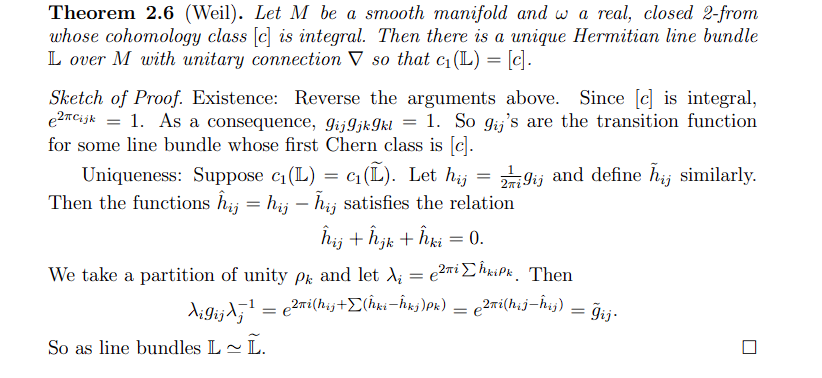
\includegraphics[width=1.0\linewidth]{屏幕截图 2024-12-17 180658.png}
  \caption{Proof}
\end{figure}





\begin{thebibliography}{99}


    \bibitem[Jos]{Jos}
      A. Joseph. \textit{On the associated variety of a primitive ideal}, J. Algebra. \textbf{93} (1985), no. 2, 509-523.


    \bibitem[BB]{BB}
      W. Borho, J. Brylinski. \textit{Differential operators on homogeneous spaces I: irreducibility of the associated variety}, Inv. Math. \textbf{69} (1982), 437-476.

    \bibitem[KV]{KV} 
      W. Knapp and D. Vogan, \textit{Cohomological Induction and Unitary Representations}, Princeton Mathematical Series, vol. 45, Princeton University Press, Princeton, NJ, 1995.
    \bibitem[SGA3]{SGA3}
      M. Demazure, A. Grothendieck: Schémas en Groupes (SGA3) I, II, III, Lecture Notes in Mathematics 151, 152, 153, Springer, New York (1970). 


\end{thebibliography}




\end{document}



